
\documentclass[tikz,border=10pt]{standalone}
\usepackage{stanli}
\usetikzlibrary{calc}


\begin{document}


\setcoords{0}{0}[0.4][0.4][0.4]
\setaxis{1}

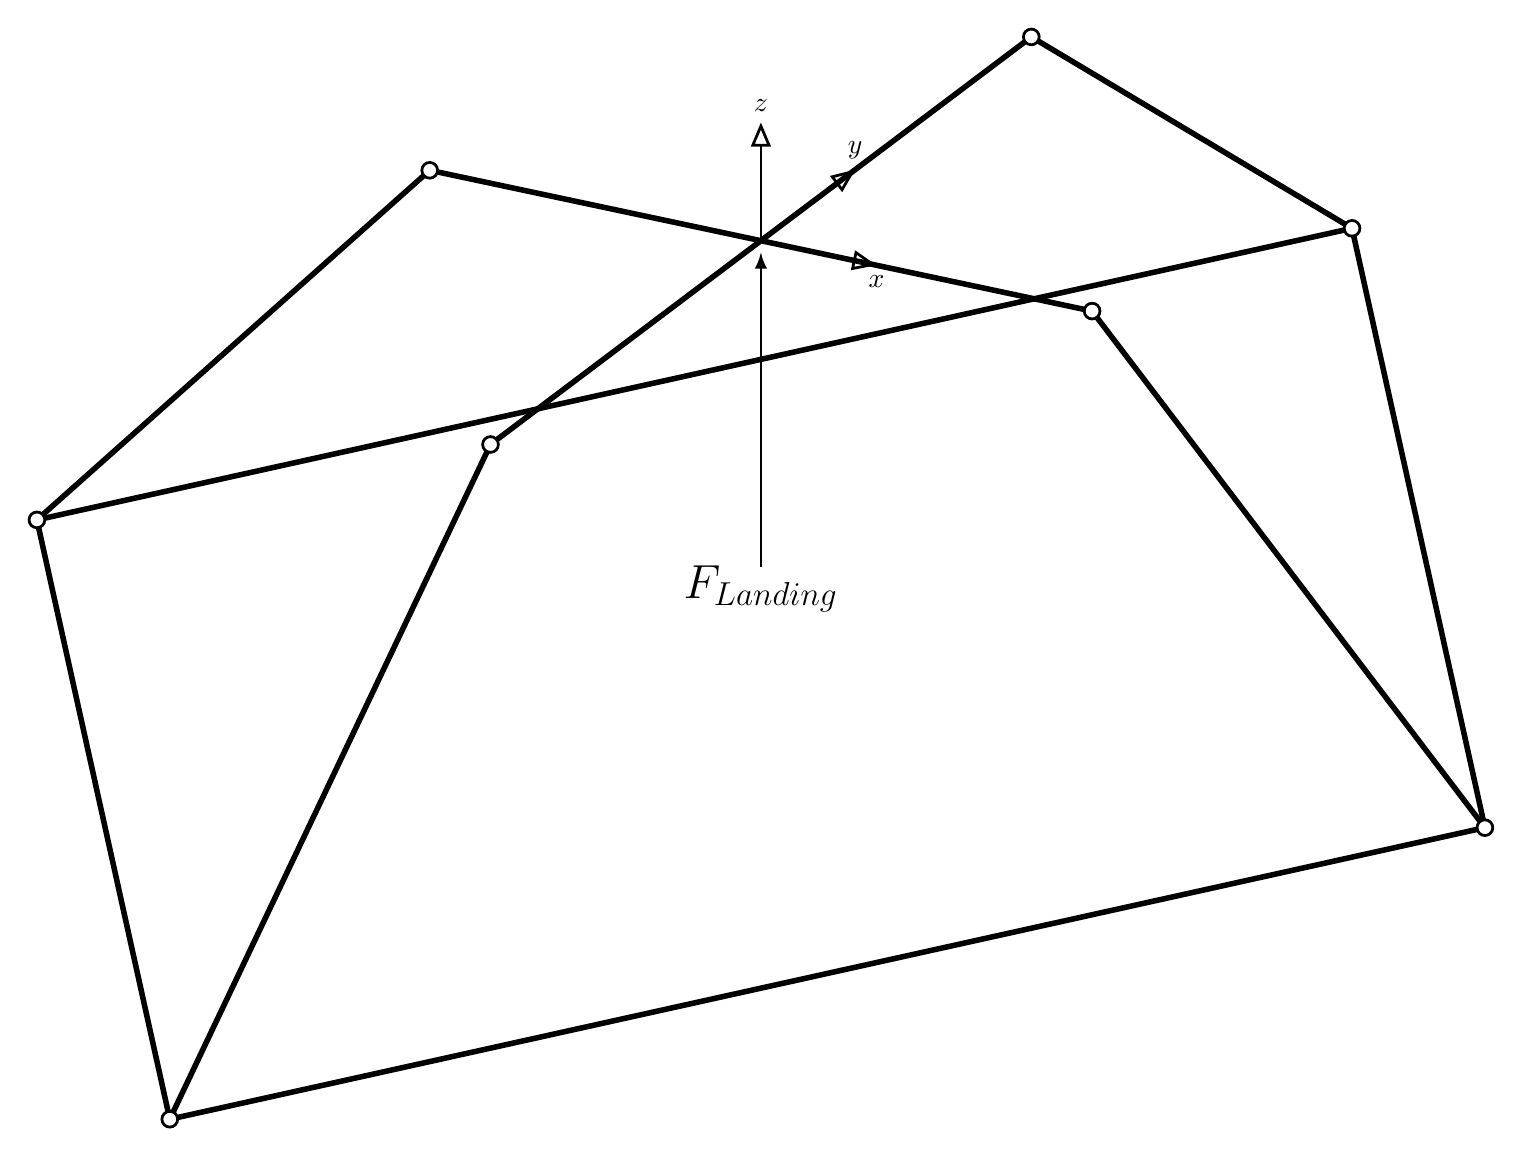
\begin{tikzpicture}[coords]
	
	\def \y {4.3}
	\def \ly {9.4}
	\def \lz {-5.5}

    
    
    \dpoint{yp} {0}{\y}{0};
    \dpoint{yn} {0}{-\y}{0};
    \dpoint{xp} {\y}{0}{0};
    \dpoint{xn}	{-\y}{0}{0};
    \dpoint{lyp} {0}{\ly}{\lz};
    \dpoint{lyn} {0}{-\ly}{\lz};
    \dpoint{lxp} {\ly}{0}{\lz};
    \dpoint{lxn}	{-\ly}{0}{\lz};
    
    
	    
    \dbeam{1}{yp}{yn};
    \dbeam{1}{xp}{xn};
    
    \dbeam{1}{xp}{lxp};
    \dbeam{1}{xn}{lxn};
    \dbeam{1}{yp}{lyp};
    \dbeam{1}{yn}{lyn};
    
    \dbeam{1}{lyp}{lxp};
    \dbeam{1}{lyn}{lxn};
    \dbeam{1}{lxp}{lyn};
    \dbeam{1}{lyp}{lxn};
    
    	
    	\dpoint{origin}{0}{0}{0};    
    \dpoint{landing_start}{0}{0}{-4};
    	\dhinge{1}{yp};
    \dhinge{1}{yn};
    \dhinge{1}{xp};
    \dhinge{1}{xn};
    \dhinge{1}{lyp};
    \dhinge{1}{lyn};
    \dhinge{1}{lxp};
    \dhinge{1}{lxn};
    
	\daxis{1}{origin};
	\dload{1}{origin}[180][1][4];
    \dnotation{1}{landing_start}{\LARGE $F_{Landing}$}[below];
    
    

\end{tikzpicture}

\end{document}
